% chktex-file 13
% chktex-file 24
% chktex-file 10
% chktex-file 17

\documentclass[../main]{subfiles}

\begin{document}

\subsection{OpenMM}\label{sec:openmm}

\subsubsection{Running out of the Box}\label{sec:openmm_ootb}

OpenMM\footnote{\url{https://github.com/openmm/openmm}} is a high performance molecular dynamics (MD) code built with a focus on GPU platforms.
The source code for OpenMM contains CUDA and OpenCL code allowing many platforms to be targeted for computation.

With OpenCL support it is possible to target Intel GPUs and run OpenMM out of the box.
This process is straightforward and comparable to other platforms.
For the readers reference OpenMM can be installed using the following command:

\begin{verbatim}
conda install -c conda-forge openmm
\end{verbatim}

OpenMM was installed on Intel DevCloud, and targeting the XeMax GPU the following simple benchmark was run:

\begin{verbatim}
python benchmark.py --test=pme --platform=OpenCL
    --precision=single --seconds=3 --heavy-hydrogens
\end{verbatim}

This yielded a simulation speed of $107 ns/day$.
For comparison, a Nvidia Quadro M1000M (a 2015 GPU with 1.6 times the thermal design power) provides simulation speeds of $82 ns/day$ in the same benchmark.
Note that instabilities where observed in these benchmarks on the Intel DevCloud with simulations longer than 3 seconds, such instabilities are not observed on other platforms.

\subsubsection{What to Port to SYCL?}\label{sec:openmm_whattoport}

MD simulations contain computations of many different forces such as those stemming from Lennard-Jones, harmonic bond or electrostatic potentials among many others.
The approach OpenMM, and many MD codes, take to computing all these forces is to write separate kernels and code to compute each force and then to sum the force on each atom after the individual calculations are complete.
This separation of the kernels allows for a port to consider one kernel at a time.
We chose this strategy for simplicity and to further simplify we opted to port the code within OpenMM which addresses the bonded forces.
The code for the bonded forces contains the same challenges as the full source code, but is conceptually one of the most simple forces.

\subsubsection{How to Port to SYCL?}\label{sec:openmm_howtoport}

The GPU specific code in OpenMM uses what is referred to as a common compute framework.
The main kernels of the code are written in a platform agnostic form and these are then assembled at run time for the target platform.
This run time code generation presented significant challenges to porting OpenMM to SYCL.
The first challenge was that the application of conversion tools such as the Intel DPC++ Compatibility Tool was difficult.
We found it was not possible to convert the CUDA source code to SYCL in our testing as the compatibility tool is not compatible with CUDA run time compilation.
If parts of the CUDA run time compilation API are passed to the compatibility tool errors are generated e.g.

\begin{verbatim}

  /*
DPCT1007:0: Migration of this CUDA API is not supported by the Intel(R) DPC++
Compatibility Tool.
*/
  nvrtcCreateProgram(&prog,      // prog
                     saxpy,      // buffer
                     "saxpy.cu", // name
                     0,          // numHeaders
                     NULL,       // headers
                     NULL);      // includeNames

\end{verbatim}


Secondly as of SYCL2020 the OpenCL interoperability APIs have been removed.
This means that the methods used for dynamic code generation in OpenMM might need more work to translate to SYCL by hand than would have been needed previously.
Since both automatic and manual translation of the dynamic code generation in OpenMM were not possible or labour intensive we instead opted to translate a kernel post dynamic generation.

\subsubsection{Porting the Generated Bonded Force Kernel}\label{sec:openmm_porting_genbf_kernel}

For simplicity we chose to port the bonded force kernel, this computes forces pertaining to the harmonic bond forces in the system.
As a starting point for this port we extracted the assembled CUDA kernel \verb!computeBondedForces()! from OpenMM.
After modifying the code to allow this extracted kernel to run in isolation the kernel was then passed through the Intel DPC++ Compatibility Tool.
Intel DPC++ Compatibility Tool was able to convert 100$\%$ of the code which could then be complied successfully without any modification.

\subsubsection{Performance of the Ported Code}\label{sec:openmm_performance}


With SYCL and CUDA versions of the bonded force kernel we compared the performance of these to codes.
To make this comparison we used XeMax GPUs on the Intel DevCloud and a local Nvidia Quadro M1000M to compute the energies of progressively larger sets of bonds.
These runs were timed and the resulting the data plotted in figure~\ref{fig:openmm}.
All the code used to generate this plot can be found here: \url{https://github.com/adw62/HarmonicBond_CUDA2SYCL}.
The results in figure~\ref{fig:openmm} demonstrate the code is running roughly as expected but more specific assertions about relative performance are not possible due to 1) the inequality of the hardware and 2) the lack of optimisation in SYCL code.

\begin{figure}[!htbp]
	\caption{Comparison of compute time for different sized sets of bonds using Intel XeMax and Nvidia Quadro M1000M. The timing runs are repeated 5 times, the line is plotted as the average of these repeats and the shaded areas as $\pm$ the standard deviation of the repeats.}
	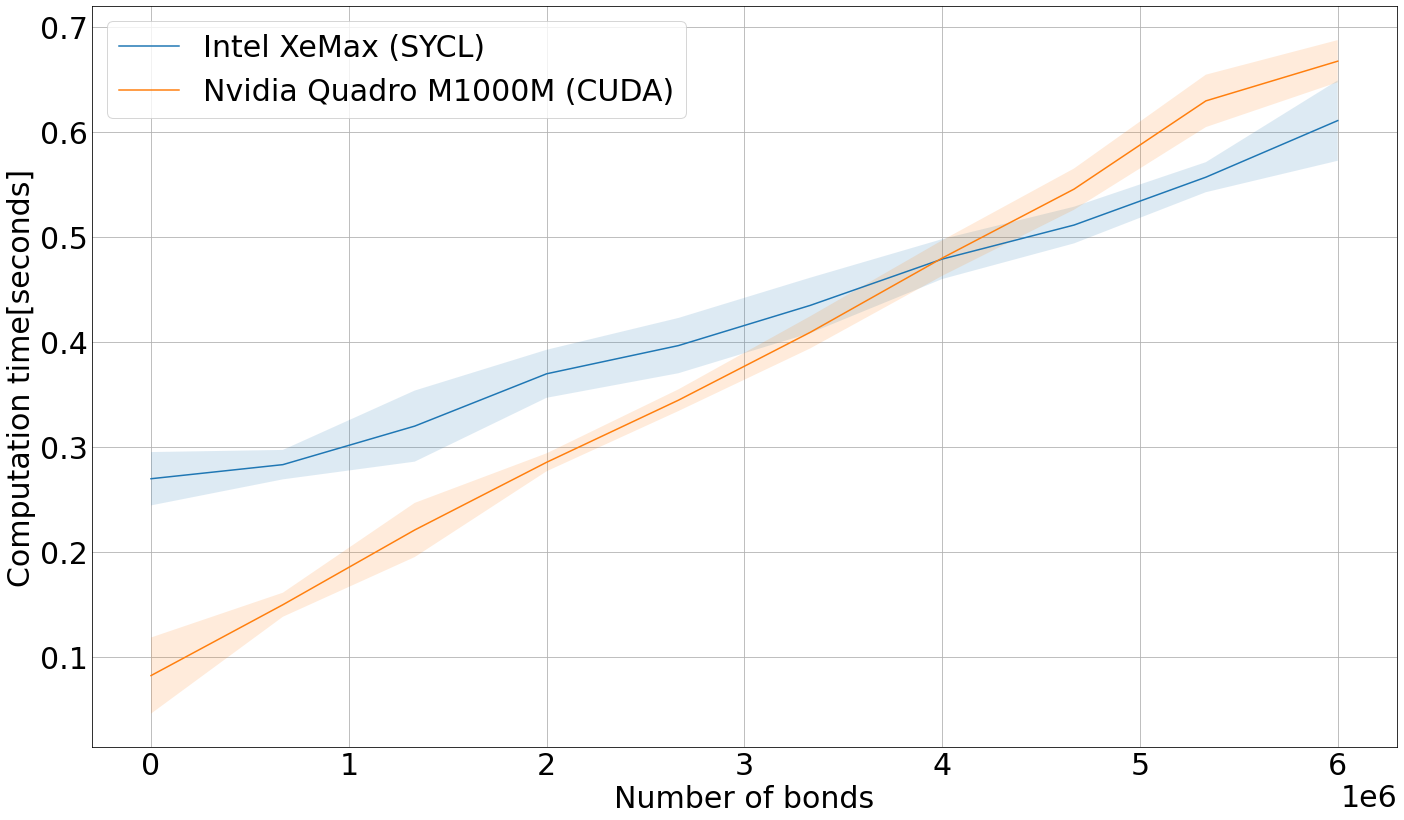
\includegraphics[width=0.75\textwidth]{openmm2.png}
	\label{fig:openmm}
\end{figure}

\subsubsection{Further Work for Porting OpenMM}\label{sec:openmm_furtherwork}

As has already been mentioned above there are two major parts of an OpenMM port to SYCL that have not addressed in this work these are 1) porting of all force kernels and 2) porting of dynamic code generation methods.
Before continuing to port more force kernels it is the opinion of the authors that porting of the dynamic code generation should be the next priority.
The authors are aware of other codes which use run time compilation with SYCL (https://github.com/ginkgo-project/ginkgo) and so although porting OpenMM to SYCL would take significant effort to perform manually we are not aware of any reasons why it would not be possible.


\subsubsection{Effort Required for Porting OpenMM}\label{sec:openmm_effort}

The authors of this section were novices in CUDA programming and new to SYCL programming as such the results here should represent the effort required for a port to be achieved by user new to GPU programming.
Porting of the bonded kernel can be considered as three tasks 1) learning sufficient CUDA to understand the problem and 2) converting the extracted code using the Intel compatibility tool.
The authors estimate that task 1) was the most time consuming with a rough estimate of 1--2 PM (person-month) but task 2), once the CUDA kernel was in hand and well understood, was much faster and took on the order of 0.25 PM.
From the perspective of a GPU programming novice we comment that the porting of a single kernel from CUDA to SYCL was very straight forward provided the CUDA API in the code being ported is supported.
We have found in this part of the work sections of the CUDA API that are not supported, namely nvrtc.
Without the support of Intel compatibility tool it is the opinion of this author that the complexity to port a code such as OpenMM is well beyond what is possible for a novice.

\end{document}
